\documentclass[lecture.tex]{subfiles}

\begin{document}


\exercice{}
%\video{https://youtu.be/blablabla}
\enonce{rdm-0014}{Etude de poutres de section rectangulaire}

On considère les deux poutres ci-dessous soumisent à  un  effort  tranchant $M_{fz}$ identique.

\begin{center}
  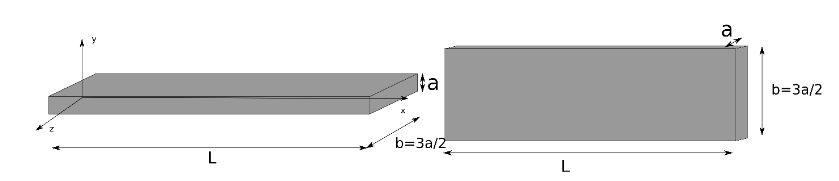
\includegraphics[scale=0.5]{exo-poutre-section-rectangle.png}
\end{center}

\begin{enumerate}
  \item Sur quelle surface les contraintes sont maximales.
  \item Donner le moment quadratique $I_z$ pour les deux poutres. (l’axe $x$  est confondu avec la fibre neutre de la poutre).
  \item Sous  un  effort  tranchant  identique,  laquelle  des  deux  poutres  fléchira  le  plus. Justifier votre réponse.
\end{enumerate}


\finenonce{rdm-0014}
\finexercice


\end{document}
